Shortest path algorithms are of central importance in Computer Science.
A particularly fascinating aspect of these algorithms is
that they can often be generalised to rather exotic algebraic structures
such as \emph{semirings}~\cite{gondran_graphs_2008}.
A semiring $\langle S, \oplus, \otimes, 0, 1 \rangle$ is
comprised of a commutative monoid $\langle S, \oplus, 0\rangle$
and a monoid $\langle S, \otimes, 1\rangle$ such that
two \emph{distributivity axioms} hold:
for all $a, b, c \in S$,
\begin{equation}
\label{eq:left:distributivity}
    a\otimes (b \oplus c) = (a\otimes b) \oplus (a\otimes c),
\end{equation}
\begin{equation}
\label{eq:right:distributivity}
    (b \oplus c) \otimes a = (b\otimes a) \oplus (c\otimes a).
\end{equation}

In this generalised, algebraic setting a directed graph having $n$ nodes and arc weights in $S$
can be represented as a $n\times n$-matrix $\mathbf{A}$ over $S$, the graph's
adjacency matrix.
Given a path $p = v_0, v_1, \ldots, v_k$---a sequence of nodes--- its \emph{weight}
is defined as
\begin{equation}
\label{eq:def:weight}
    w_{\mathbf{A}}(p)
    \equiv
    \mathbf{A}(v_0,\ v_1)
    \otimes \mathbf{A}(v_0,\ v_1)
    \otimes \cdots
    \otimes \mathbf{A}(v_{k-1},\ v_k),
\end{equation}
with the empty path assigned the weight $1$.
The generalised shortest-path problem is then to find
a matrix $\mathbf{A}^*$ such that
\begin{equation}
\label{eq:global}
\mathbf{A}^*(i,\ j) = \displaystyle\bigoplus_{p \in \pi(i,\ j)} w_{\mathbf{A}}(p)
\end{equation}
where $\pi(i,\ j)$ represents the set of all paths from node $i$ to node $j$.
Such solutions do not always exist, and \todo{SAY SOMETHING}

A nice feature of working in this generalised, algebraic setting is
the ability to vary the semiring that parameterises the algorithm.
In particular, for the reader not familiar with this generalisation,
we define the \emph{shortest path semiring} as
\begin{equation}
\label{eq:def:sp}
\mathbb{sp} \equiv \langle\mathbb{N}{\infty}, min, +, \infty, 0\rangle,
\end{equation}
where path weight is `just' the sum of arc weights.
Here, $\mathbb{N}{\infty}$ is the set of natural numbers extended with a `point
at infinity', $\infty$.
To get some feeling for the power of the
algebraic approach consider another semiring
\begin{equation}
\label{eq:def:cap}
\mathbb{cap} \equiv \langle\mathbb{N}{\infty}, max, min, 0, \infty\rangle,
\end{equation}
which can be used to compute \emph{maximum capacity paths}.
The weight of a path is determined by $min$ to be the
weight of a bottleneck arc.
The key idea here is that a generic, parametric implementation of a shortest
path algorithm can be developed and then instantiated with
different semirings, and thereafter uniformly used to calculate different properties
of graphs.
The interested reader can find a thorough treatment of
this material in~\cite{gondran_graphs_2008}.

\subsection{Dropping distributivity}
\label{subsect.dropping.distributivity}

It is well known that if $\mathbf{A}^*$ exists, then it
is a solution of the (left) equation
\begin{equation}
\label{eq:left:local}
\mathbf{L} = (\mathbf{A}\otimes \mathbf{L}) \oplus \mathbf{I}
\end{equation}
as well as the (right) equation
\begin{equation}
\label{eq:right:local}
\mathbf{R} = (\mathbf{R}\otimes \mathbf{A}) \oplus \mathbf{I}.
\end{equation}

The distributivity axioms,
Equations~\ref{eq:left:distributivity} and~\ref{eq:left:distributivity},
are essential in the semiring theory outlined above.
Thus it may seem suprising that recent research has shown that
the matrix equations ~\ref{eq:left:local} and ~\ref{eq:right:local}
can sometimes be solved even if when
distributivity axioms do not hold in the algebraic structure employed.
Much of this work was originally motivated
by investigations of the Border Gateway Protocol (BGP),
the Internet routing protocol which has evolved to
maintains global connectivity between Internet Service Providers (ISPs).
In BGP the anologue of the weight of a path
$p = v_0, v_1, \cdots,\ v_k$ at node $v_0$
is dominated by the contractural relationships between
the networks associated with nodes $v_0$ and $v_1$.
The typical relationships involve those between customers
and providers and between competing ISPs (that must exchange
routing information in order to provide connectivty to
the global Internet).

But how can we interpret such solutions?
Take Equation~\ref{eq:left:local} for example.
If we assume that $\mathbf{L}$ solves this equation
and that $i \neq j$, then we have
\begin{equation}
\label{eq:left:local:at:i}
\mathbf{L}(i,\ j) = \displaystyle\bigoplus_{q \in N(i)} \mathbf{A}(i,\ q) \otimes \mathbf{L}(q,\ j),
\end{equation}
where $N(i)$ is the set of neighbors of node $i$.
We can interpret this from node $i$'s perspective as
the best path weight available given the paths its neighbors
have obtained.
That is, $\mathbf{L}$ does not represent the globally optimal
path weights, but rather an equilibrium point that we will
call \emph{locally optimal}.

\subsection{Generalising Dijkstra's algorithm}

\begin{figure}[ht]
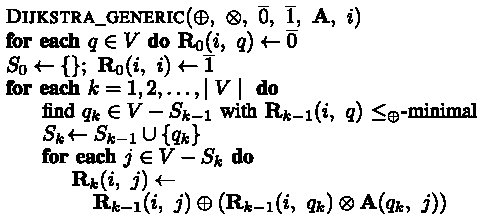
\includegraphics{algorithm.pdf}
\caption{Dynerowicz and Griffin's imperative generalised Dijkstra's algorithm}
\label{fig.algorithm}
\end{figure}

\todo{finish me}

\subsection{Agda}
\label{subsect.agda}

Agda~\cite{norell_dependently_2009} is a dependently-typed functional programming language \emph{cum} proof assistant for higher-order intuitionistic logic.
In contrast to similar systems, such as Coq~\cite{bertot_short_2008} and Matita~\cite{asperti_matita_2011}, proof terms are constructed by hand via a process of type-directed refinement, rather than being constructed via tactic-assisted metaprogramming.

Agda has a uniform syntax that should be familiar to Haskell programmers and users of other dependently-typed proof assistants.
One syntactic novelty is a flexible system of user-declared Unicode mixfix identifiers~\cite{danielsson_parsing_2011} with `holes' in an identifier being denoted by underscores.

We write \AgdaSymbol{(}\AgdaBound{x}~\AgdaSymbol{:}~\AgdaBound{A}\AgdaSymbol{)}~\AgdaSymbol{→}~\AgdaBound{B} for the dependent function space where \AgdaBound{x} may occur in \AgdaBound{B}, and write \AgdaBound{A}~\AgdaSymbol{→}~\AgdaBound{B} when \AgdaBound{x} does not occur in \AgdaBound{B} as is usual.
We enclose arguments to be inferred in braces, as in \AgdaSymbol{\{}\AgdaBound{x}~\AgdaSymbol{:}~\AgdaBound{A}\AgdaSymbol{\}}~\AgdaSymbol{→}~\AgdaBound{B}, sometimes making use of the shorthands \AgdaSymbol{∀}~\AgdaBound{x}~\AgdaSymbol{→}~\AgdaBound{B} and \AgdaSymbol{∀}~\AgdaSymbol{\{}\AgdaBound{x}\AgdaSymbol{\}}~\AgdaSymbol{→}~\AgdaBound{B} when types can be inferred.
We write \AgdaDatatype{Σ}~\AgdaBound{A}~\AgdaBound{B} for the dependent sum type whose first projection has type \AgdaBound{A}, and write \AgdaBound{A}~\AgdaDatatype{×}~\AgdaBound{B} when the second projection does not depend on the first, as is usual.
Dependent sums are constructed using the comma constructor: \AgdaBound{x}~\AgdaInductiveConstructor{,}~\AgdaBound{y}.
We sometimes write \AgdaFunction{∃}~\AgdaSymbol{λ}~\AgdaBound{x}~\AgdaSymbol{→}~\AgdaBound{P} for the dependent sum type when the type of the first projection can be inferred.
Propositional equality between two types is written \AgdaBound{A}~\AgdaDatatype{≡}~\AgdaBound{B} and has a single canonical inhabitant, \AgdaInductiveConstructor{refl}.
Lastly, we write \AgdaBound{A}~\AgdaDatatype{⊎}~\AgdaBound{B} for the disjoint union type with constructors \AgdaInductiveConstructor{inj₁} and \AgdaInductiveConstructor{inj₂} and \AgdaFunction{¬}~\AgdaBound{A} for constructive negation.

Agda is a predicative type theory with an infinite universe hierarchy, \AgdaPrimitiveType{Setᵢ}, with \AgdaPrimitiveType{Set}---the type of small types---being identified with \AgdaPrimitiveType{Set₀}, the base universe in Agda's hierarchy.
As a matter of course universe \AgdaPrimitiveType{Setᵢ} is not automatically contained in \AgdaPrimitiveType{Setⱼ} when $i < j$ and requires explicit lifting with \AgdaFunction{Lift}.
Universe polymorphism is used extensively throughout this development, with explicit quantification over universe levels.

%\paragraph{Contributions and map of paper}
%\subsection{Map of Paper}
%\label{subsect.map.of.paper}
%In Section~\ref{sect.basic.definitions} we cover some definitions needed to define Dijkstra's algorithm and its correctness proof.
%In Section~\ref{sect.path.algebras.their.properties.and.models} we discuss `path algebras', a variety of algebraic structure central to our proof of correctness, also providing three models of path algebras to demonstrate that models exist and that path algebras are not categorical.
%In Section~\ref{sect.dijkstras.algorithm.and.its.correctness} we discuss the imperative Dijkstra algorithm, our functional implementation, and main body of the correctness proof leading up to our main theorem: Dijkstra's algorithm computes a right-local solution.
%In Section~\ref{sect.example} we demonstrate the algorithm in action with an example execution inside Agda.
%In Section~\ref{sect.conclusions} we conclude.
